\chapter{Rapport intermédiaire : 10.11.2018 au 23.11.2018}

\section{Collecte des données}
La collecte des données est un point important de ce travail. Il a été nécessaire de réfléchir quoi prendre et de quel manière. Pour ce faire, Michael Muller qui avait réalisé sa thèse de master concernant le positionnement indoor a réalisé un programme python fonctionnant sur PC et permettant de récupérer les mesures. Ci-dessous sera détaillé un peu plus précisément ce programme afin de pouvoir le prendre en main et réaliser les prises de mesures. 

Ci-dessous, il sera également précisé comment les données ont été structurée afin de pouvoir être utilisée plus tard dans un algorithme d'apprentissage. 

Finalement il sera détaillé comment les mesures ont été effectuées selon le plan du laboratoire.

\subsection{Programme de prise de mesure}
\subsubsection{Architecture}
\subsubsection{Modification du programme original}

\cite{MIC}

\subsection{Structure des données}

\subsection{Plan de mesure}

%\begin{lstlisting}
% for i=0 to Array.length(t)-1 do
%\end{lstlisting}


%\begin{enumerate}
%	\item fgfd
%	\item gdgfd
%\end{enumerate}


%\begin{figure}[H]
%	\begin{center}
%		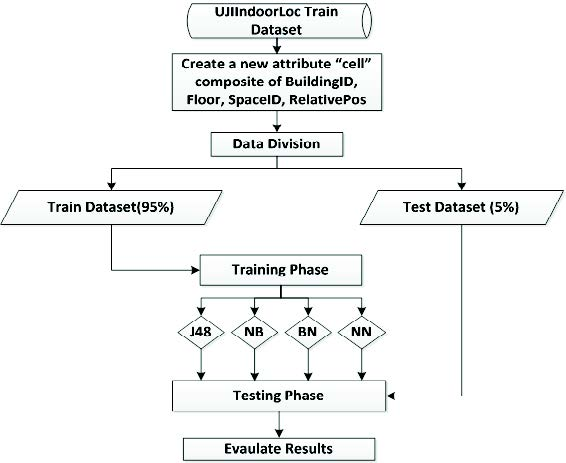
\includegraphics[scale=1]{figures/newattribute.jpg}
%		\caption{The new attribute “cell” construction phase}
%		\label{fig:newAttribute} %% NOTE: always label *after* caption!
%	\end{center}
%\end{figure}

%\todo{Compléter cette partie qui semble importante}

